% Provenance (never printed): sources/book2/BRIEFS.md, g12-03. The quantity equation and its growth-rate form; the record
% across countries; hyperinflations and how they ended; the costs of inflation; nominal and real rates (Fisher). Real numbers:
% figdata/grade-12/03-inflation-and-money/ (WDI broad money growth, CPI inflation, GDP growth, 1990-2019, 123 countries; JST
% velocity, USA 1960-2020). Ledger: Hanke-Krus table page, Wikipedia on Zimbabwe and on the pengő, Econlib on Germany
% 1921-23, Brunnermeier et al. 2024 abstract, Book 1's Rentenmark rows. The Hanke-Krus table itself (cato.org, 403) was not
% read: no peak monthly rate is printed. Photograph: a Hungarian 1946 note (Commons, PD; Book 1 prints the German one). Kestria's numbers are invented.
\chapter{Inflation and the Quantity of Money}\label{ch:g12:inflation-and-money}

From 1990 to 2019, Japan's \omterm{def:g11:money-and-banking:broad-money}{broad money} grew by 2.0\,\% a year on average, and its prices by 0.5\,\%. Brazil's money grew by 73\,\% a year and its prices by 68\,\%. In the
Democratic Republic of the Congo, money grew by 149\,\% a year and prices by 173\,\%. Across 123 countries with the data, the correlation between average money growth and
average inflation over those thirty years is 0.97.
% figdata: qtm (JPN 1.96/0.47, BRA 73.45/67.97, COD 148.74/172.83); qtm_key (n 123, corr 0.968)

Over long periods, and above all where inflation is high, prices rise about as fast as money grows. This chapter derives that from an identity, shows where it holds and
where it does not, follows the hyperinflations that are its most extreme cases, and asks who pays for inflation.

\begin{openingchart}{Average yearly growth of broad money against average yearly consumer price inflation, 123 countries, 1990--2019 (countries with at least 25 years of
both), logarithmic scales. The line marks equal rates.}{World Bank, World Development Indicators (FM.LBL.BMNY.ZG, FP.CPI.TOTL.ZG)}
\begin{tikzpicture}
\begin{axis}[omscatter, width=0.8\linewidth, height=6.4cm, xmode=log, ymode=log, xmin=1, xmax=250, ymin=0.3, ymax=250, log ticks with fixed point,
  xtick={1,2,5,10,20,50,100,200}, ytick={0.5,1,2,5,10,20,50,100,200}, xlabel={money growth, per cent a year}, ylabel={inflation, per cent a year}]
\addplot+[omDef, mark=*, mark size=1.2pt, only marks] table[x=money, y=infl] {figdata/grade-12/03-inflation-and-money/out/qtm.csv};
\addplot[gray, dashed, sharp plot, no marks, domain=1:250, samples=2] {x};
\node[font=\scriptsize, anchor=east] at (axis cs:140,172.83) {Congo, D.R.};
\node[font=\scriptsize, anchor=north west] at (axis cs:73.45,67.97) {Brazil};
\node[font=\scriptsize, anchor=north] at (axis cs:1.96,0.47) {Japan};
\end{axis}
\end{tikzpicture}
\end{openingchart}

\begin{recall}
From the grades 6--9 volume: the inflation rate, real and nominal values, hyperinflation and the German one of 1923. From \cref{ch:g10:price-indices}: the \omterm{def:g10:price-indices:real-interest-rate}{real interest
rate}. From \cref{ch:g11:money-and-banking}: \omterm{def:g11:money-and-banking:reserves}{central bank money} and \omterm{def:g11:money-and-banking:broad-money}{broad money}. From the mathematics volumes: the logarithm, which turns products into sums.
\end{recall}

\section{The quantity equation}\label{sec:g12:inflation-and-money:equation}

\begin{definition}[Velocity of money]\label{def:g12:inflation-and-money:velocity}
The \emph{velocity of money}\index{velocity of money} is \omterm{def:g10:national-accounts:nominal-gdp}{nominal GDP} divided by the quantity of money: $V = PY/M$, the number of times a year an average unit of money is
spent on final output.
\end{definition}

\begin{definition}[Quantity equation]\label{def:g12:inflation-and-money:quantity-equation}
The \emph{quantity equation}\index{quantity equation} is $MV = PY$: money times velocity equals the price level times real output.
\end{definition}

As written it is an identity: it holds whatever happens, because velocity is defined to make it hold. It becomes a theory once one says something about how $V$ and $Y$
move.

\begin{proposition}[The growth-rate form]\label{prop:g12:inflation-and-money:growth}
Write $g_X = \ln X_{t+1} - \ln X_t$ for the logarithmic growth rate of a positive quantity $X$. Then $g_M + g_V = g_P + g_Y$. For growth rates of a few per cent, these are close
to ordinary percentage growth rates, and inflation is approximately money growth plus velocity growth minus output growth.
\end{proposition}
\begin{proof}
Taking logarithms of $M_tV_t = P_tY_t$ at two dates gives $\ln M_t + \ln V_t = \ln P_t + \ln Y_t$ for each $t$; subtracting the equation at $t$ from that at $t + 1$ gives the
result. For a growth rate $x$, $\ln(1 + x) \approx x$ when $x$ is small, since the derivative of $\ln$ at 1 is 1.
\end{proof}

\begin{model}{The quantity theory of money}
\assumes Velocity is stable or changes slowly; real output grows at a rate set by labour, capital and technology, not by money; the central bank sets money growth.
\predicts Over long periods, inflation is about money growth minus output growth; a country that grows money ten points faster has about ten points more inflation.
\tested Consistent with it: across 123 countries from 1990 to 2019, averages of money growth and inflation line up close to the line of equal rates (the opening chart), with a correlation of
  0.97; the fit is tightest where inflation is high.
\breaks Where inflation is low and over short periods, velocity moves as much as money: in the United States it fell from 1.98 in 2007 to 1.44 in 2019 (the chart below).
  In a hyperinflation it rises as people get rid of money.
\end{model}
% figdata: qtm_key (corr 0.968); velocity (2007 1.98, 2019 1.44)

\begin{omchart}{Velocity of broad money in the United States, nominal GDP divided by broad money, 1960--2020.}{Jordà--Schularick--Taylor Macrohistory Database}
\begin{tikzpicture}
\begin{axis}[omtime, width=0.8\linewidth, height=5.0cm, xmin=1960, xmax=2020, ymin=1, ymax=2.4, xtick={1960,1970,...,2020}, ylabel={velocity, per year},
  y tick label style={/pgf/number format/.cd, fixed, precision=1}]
\addplot[omDef, thick] table[x=year, y=v] {figdata/grade-12/03-inflation-and-money/out/velocity.csv};
\end{axis}
\end{tikzpicture}
\end{omchart}
% figdata: velocity (1960 1.78, 1997 2.19 peak, 2020 1.18)

\section{Hyperinflations}\label{sec:g12:inflation-and-money:hyper}

\begin{definition}[Seigniorage and the inflation tax]\label{def:g12:inflation-and-money:seigniorage}
\emph{Seigniorage}\index{seigniorage} is the revenue a government gets from issuing money: the new money it creates in a period, valued at the prices of the start of the
period. The \emph{inflation tax}\index{inflation tax}\phantomsection\label{def:g12:inflation-and-money:inflation-tax} is the loss of real value that inflation inflicts
on those who hold money: at inflation $\pi$, money held through a period loses a fraction $\pi/(1 + \pi)$ of its purchasing power.
\end{definition}

A government that cannot borrow or tax enough can have its central bank buy its debt with new money. With real money balances $m = M/P$ held steady and money growing by
$\mu$ a period, \omterm{def:g12:inflation-and-money:seigniorage}{seigniorage} is $\mu m$ a period. The trouble is that people hold less money when it loses value fast; velocity rises and real balances fall, so the same
revenue needs ever faster money growth.

\begin{omfigure}
\renewcommand{\arraystretch}{1.25}
\begin{tabular}{l|r@{\hspace{2.5em}}l|r}
\multicolumn{4}{c}{\textbf{The central bank}} \\
\multicolumn{2}{c|}{assets} & \multicolumn{2}{c}{liabilities} \\ \hline
government \omterm{def:g12:present-value:bond}{bonds} & $+50$ & government's account & $+50$ \\
 & & then: banks' reserves & $+50$ \\
 & & \phantom{then:} government's account & $-50$ \\
\end{tabular}

\medskip
{\small A deficit paid with new money. The central bank buys 50 of government \omterm{def:g12:present-value:bond}{bonds} and credits the government's account; when the government pays its employees and
suppliers, the money moves to their banks as reserves, and to their accounts as deposits. \omterm{def:g11:money-and-banking:reserves}{Central bank money} and \omterm{def:g11:money-and-banking:broad-money}{broad money} have both risen by 50.}
\end{omfigure}

\begin{record}[Germany, 1922--23]
% ledger: g12:germany-1922, g8:rentenmark-issue, g8:rentenmark-rate
The Reichsbank bought the government's debt with newly printed money: its holdings of bills rose from 922 million marks in December
1921 to 6.6 billion in July 1922. In May 1922 only 21\,\% of the government's income came from taxes; in July prices rose by 50\,\% in a single month. The end came in
November 1923: a new currency, the Rentenmark, went into circulation on 15 November, worth one trillion old marks, and the government's borrowing through Treasury bills
discounted at the central bank was to cease; the government also planned to dismiss a quarter of its employees over four years.
\end{record}

In Hungary in 1946, at one stage prices doubled in about fifteen hours. The forint, introduced on 1 August 1946, replaced $4 \times 10^{29}$ pengő.
% ledger: g12:pengo

\begin{omfigure}
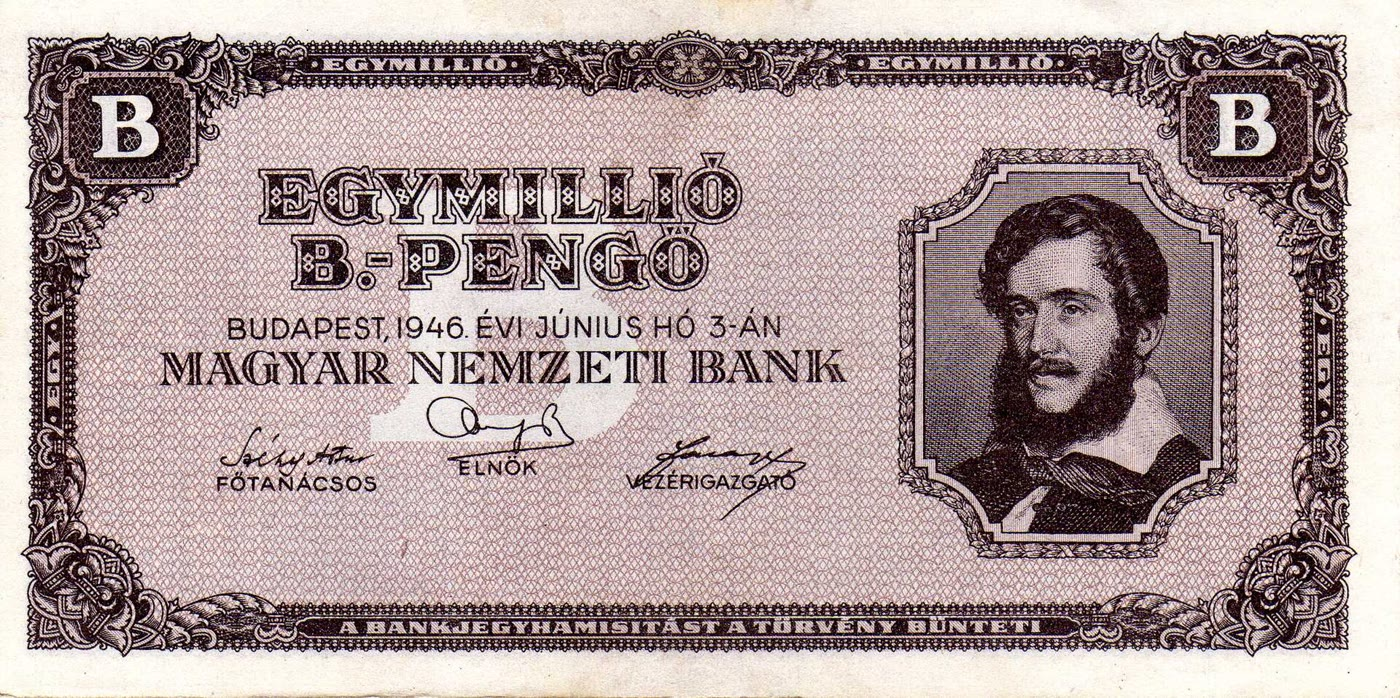
\includegraphics[width=0.58\linewidth]{images/book2/photos/g12-inflation-pengo-1946.jpg}

{\small A Hungarian note for one million B.-pengő, dated 3 June 1946. One B.-pengő was a million million pengő, so the note stood for $10^{18}$ pengő.}
\end{omfigure}

\begin{record}[Zimbabwe, 2007--09]
% ledger: g12:zimbabwe
The government of Zimbabwe printed money to finance military involvement in the Democratic Republic of the Congo and higher pay for soldiers and officials. One estimate put
the rise in prices over the year to mid-November 2008 at 89.7 sextillion per cent, about $9 \times 10^{22}$\,\%. In April 2009 Zimbabwe stopped printing its currency, and
the currencies of other countries were used instead.
\end{record}

\begin{measure}[Measuring inflation in a hyperinflation]
% ledger: g12:hanke-method
When prices change by the hour, official price surveys fall behind, and some governments stop publishing them. One widely used table of hyperinflations counts an episode
from the first month in which prices rise by 50\,\% or more, and where official figures are missing or suppressed it estimates inflation from black-market exchange rates
against a stable currency, on the reasoning that, over months, the prices of traded goods follow the exchange rate.
\end{measure}

Each ended with a break: in Germany a new currency and the end of the government's borrowing from the central bank; in Hungary a new currency; in Zimbabwe the end of
its own currency. The logic of \omterm{def:g12:inflation-and-money:seigniorage}{seigniorage} says why a new currency alone is not enough: as long as new money pays for a deficit, it keeps being printed, so the deficit
itself has to close, by taxes, spending cuts or help from abroad.

\section{The costs of inflation}\label{sec:g12:inflation-and-money:costs}

\begin{definition}[Unexpected inflation]\label{def:g12:inflation-and-money:unexpected-inflation}
\emph{Unexpected inflation}\index{unexpected inflation} is the difference between actual inflation and the inflation people expected when they signed contracts fixed in
money.
\end{definition}

Expected inflation can be built into wages, prices and interest rates; it still has costs: people hold less money and make more trips to the bank, firms change price lists
more often, and taxes levied on nominal gains tax gains that are not real. \omterm{def:g12:inflation-and-money:unexpected-inflation}{Unexpected inflation} redistributes: it lowers the real value of debts fixed in money, so it moves
\omterm{def:g11:inequality:wealth}{wealth} from lenders to borrowers, and from those whose pay is fixed to those who pay them. In the German inflation of 1919--1923, inflation sharply lowered firms' real
debt burdens and bankruptcies, and firms with more debt in marks benefited most.
% ledger: g12:debt-inflation

\section{Nominal and real interest rates}\label{sec:g12:inflation-and-money:fisher}

\begin{definition}[Fisher effect]\label{def:g12:inflation-and-money:fisher-effect}
The \emph{Fisher effect}\index{Fisher effect} is the rise of nominal interest rates one for one with expected inflation, leaving the expected real rate unchanged: with
nominal rate $i$, real rate $r$ and expected inflation $\pi^e$, $1 + i = (1 + r)(1 + \pi^e)$, so that $i \approx r + \pi^e$.
\end{definition}

A lender who wants a real return of 3\,\% and expects 2\,\% inflation asks about 5\,\%; if she expects 10\,\%, she asks about 13\,\%. When inflation turns out higher than
expected, the real rate actually paid is lower than intended: that is the redistribution of the previous section, seen from the lender's side.

\section{Exercises}

\begin{exercise}[$\star$]\label{exo:g12:inflation-and-money:1}
Money is 200, velocity 5 and real output 500. Find the price level.
\end{exercise}

\begin{exercise}[$\star$]\label{exo:g12:inflation-and-money:2}
\omterm{def:g10:national-accounts:nominal-gdp}{Nominal GDP} is 3000 and money 600. Find velocity. If money doubles and velocity and real output do not change, what happens to the price level?
\end{exercise}

\begin{exercise}[$\star$]\label{exo:g12:inflation-and-money:3}
Money grows by 8\,\% a year, velocity is constant and output grows by 3\,\%. Find inflation approximately.
\end{exercise}

\begin{exercise}[$\star$]\label{exo:g12:inflation-and-money:4}
From the opening chart, where do Japan and the Democratic Republic of the Congo lie relative to the line of equal rates? What does that say about their velocity or output?
\end{exercise}

\begin{exercise}[$\star$]\label{exo:g12:inflation-and-money:5}
From the opening chart, are most countries above or below the line of equal rates? Explain with the growth-rate form.
\end{exercise}

\begin{exercise}[$\star\star$]\label{exo:g12:inflation-and-money:6}
In the United States, \omterm{def:g10:national-accounts:nominal-gdp}{nominal GDP} was 14\,474 billion dollars in 2007 and 21\,373 billion in 2019, and \omterm{def:g11:money-and-banking:broad-money}{broad money} 7294 billion and 14\,837 billion. Compute velocity in each
year.
% figdata: qtm_us (gdp 14474.2, 21372.6; money 7294.47, 14836.50)
\end{exercise}

\begin{exercise}[$\star\star$]\label{exo:g12:inflation-and-money:7}
Brenland's \omterm{def:g10:national-accounts:nominal-gdp}{nominal GDP} is 2400 and its money 800. Find velocity. Money rises to 1000; velocity and real output do not change. By how much do prices rise?
\end{exercise}

\begin{exercise}[$\star\star$]\label{exo:g12:inflation-and-money:8}
Money grows by 30\,\% a year, output by 2\,\%, and velocity is constant. Find inflation exactly and with the approximation.
\end{exercise}

\begin{exercise}[$\star\star$]\label{exo:g12:inflation-and-money:9}
Real money balances are 40 and money grows by 5\,\% a month, with real balances steady. Find \omterm{def:g12:inflation-and-money:seigniorage}{seigniorage} per month.
\end{exercise}

\begin{exercise}[$\star\star$]\label{exo:g12:inflation-and-money:10}
The nominal rate is 7\,\% and expected inflation 4\,\%. Find the real rate exactly and approximately.
\end{exercise}

\begin{exercise}[$\star\star$]\label{exo:g12:inflation-and-money:11}
From the velocity chart, give velocity in 1960, at its highest and in 2020.
\end{exercise}

\begin{exercise}[$\star\star\star$]\label{exo:g12:inflation-and-money:12}
From 2007 to 2019, American \omterm{def:g11:money-and-banking:broad-money}{broad money} doubled while consumer prices rose by about 24\,\%. Does this contradict the quantity theory? Use the growth-rate form and the
velocity chart.
% figdata: qtm_us (money x 2.03; cpi 153.916 -> 190.248, +23.6 %)
\end{exercise}

\begin{exercise}[$\star\star\star$]\label{exo:g12:inflation-and-money:13}
Compute the \omterm{def:g12:inflation-and-money:seigniorage}{inflation tax} rate $\pi/(1 + \pi)$ for $\pi = $ 20\,\%, 100\,\% and 1000\,\% a month. What is its limit as inflation grows, and what does that imply for the
revenue a government can raise this way?
\end{exercise}

\begin{exercise}[$\star\star\star$]\label{exo:g12:inflation-and-money:14}
A borrower takes 1000 for a year at 5\,\%, both sides expecting 2\,\% inflation. Inflation turns out to be 10\,\%. Compute the real value of the repayment, in prices of the
start of the year, as expected and as it turned out. Who gains?
\end{exercise}

\begin{exercise}[$\star\star\star$]\label{exo:g12:inflation-and-money:15}
Why have hyperinflations ended with a reform of the government's finances, and not only with a new currency? Use the records of the chapter.
\end{exercise}

\section{Problem: Kestria's Printing Press}

\begin{problem}[{Weekend problem --- a deficit paid with new money}]
\label{pb:g12:inflation-and-money:1}
Kestria's real output is 100 a month and does not change. People hold money worth half a month's output: velocity is 2 a month. The government runs a deficit of 10 a month
in real terms, paid by the central bank with new money. Use the exact growth form $(1 + \pi) = (1 + \mu)(1 + g_V)/(1 + g_Y)$, with monthly rates.

\medskip
\noindent\textbf{Part I --- The steady state.}
\begin{enumerate}
\item Find real money balances $m = M/P$.
\item Find the monthly money growth $\mu$ that yields \omterm{def:g12:inflation-and-money:seigniorage}{seigniorage} of 10.
\item With velocity constant, find monthly inflation.
\item Find the \omterm{def:g12:inflation-and-money:seigniorage}{inflation tax} rate on money held through a month.
\item Is this a hyperinflation by the 50\,\% a month threshold?
\end{enumerate}

\medskip
\noindent\textbf{Part II --- The flight from money.}
\begin{enumerate}[resume]
\item People expect inflation to go on and hold less money: over one month velocity doubles to 4, while money still grows by 20\,\%. Find inflation that month.
\item Find real money balances after the doubling.
\item With money growth still 20\,\%, find the \omterm{def:g12:inflation-and-money:seigniorage}{seigniorage} collected each month afterwards.
\item What money growth would bring \omterm{def:g12:inflation-and-money:seigniorage}{seigniorage} back to 10, and what inflation would follow?
\item Explain why a government that keeps trying to collect 10 may be driven to ever faster money growth.
\end{enumerate}

\medskip
\noindent\textbf{Part III --- The stabilisation.}
\begin{enumerate}[resume]
\item The government raises taxes and cuts spending so that the deficit is zero. What money growth does it need now?
\item With money growth zero and velocity at 4, find inflation.
\item As trust returns, velocity falls back to 2 over some months. If money did not change, what would happen to prices?
\item How much new money, in real terms, can the central bank issue during that return without raising prices?
\item Why does a new currency help, if the deficit has already been closed?
\end{enumerate}

\medskip
\noindent\textbf{Part IV --- Who paid?}
\begin{enumerate}[resume]
\item A Kestrian holds 30 of money (real) through one month at 20\,\% inflation. What does she lose?
\item A firm owes a debt fixed at 1200 kests, and prices rise by 140\,\% in one month. Find the real fall of its debt.
\item A worker's wage is fixed for a month at the start. What happens to its real value in the month of Question 6?
\item Why might the quantity theory explain this episode better than it explains the United States after 2008?
\item State the result of the problem: monthly inflation in the month velocity doubles, and the \omterm{def:g12:inflation-and-money:seigniorage}{seigniorage} collected before and after, at money growth of 20\,\%.
\end{enumerate}
\end{problem}
